\chapter{Esperimenti e risultati}
\label{chap:esperimenti}


...
 - metodo, obiettivi, metriche, ambiente\&strumenti
 
La metrica utilizzata per valutare i modelli è l'accuratezza, misurata sui dati di test. 
...


Tutti gli esperimenti sono stati eseguiti su un server con CPU Intel(R) Xeon(R) W-1250P CPU @ 4.10GHz e con 31GB di ram (?? saran poi 32). Il linguaggio di programmazione utilizzato è Python 3.10.10 ed è stato utilizzato il solver Gurobi 10.0.1. 

\section{Dataset}
Nel valutare algoritmi di addestramento automatico, è di fondamentale importanza la scelta dei dataset utilizzati, dato che l'apprendimento è basato proprio su di essi. Per gli esperimenti descritti in seguito, sono stati usati due approcci nella scelta dei dataset. Il primo approccio consiste nell'utilizzo di dataset sintetici, generati specificatamente per questo lavoro. Il secondo approccio consiste nell'utilizzare dei dataset noti, tipicamente utilizzati in letteratura per valutare modelli di apprendimento automatico. Entrambi gli approcci hanno vantaggi e svantaggi. Nel primo caso, risulta molto comodo poter modificare a piacimento le caratteristiche dei dataset, per esempio per valutare l'algoritmo proposto su dataset di difficoltà crescente, oppure con quantità di rumore crescente. Lo svantaggio è che si potrebbero ottenere dei risultati poco significativi, perché ottenuti su dati generati ad hoc e quindi poco significativi per il confronto con altri modelli. Per questo ha senso utilizzare anche dataset noti, dei \textit{benchmark}, per avere risultati più robusti.

\subsubsection{Metriche dataset}
Per avere a priori un'indicazione della difficoltà del dataset, sono state considerate alcune metriche.
Con difficoltà del dataset, considerando che stiamo trattando un problema di classificazione binaria, intendiamo la difficoltà nel trovare un margine di separazione ideale. Abbiamo utilizzato quindi le metriche \textit{F1} ed \textit{F1v}.

\begin{itemize}
    \item \textbf{F1} è la sigla per la metrica \textit{Maximum Fisher’s discriminant ratio}. Questa metrica misura la sovrapposizione tra le varie feature per ogni classe.
    $$F1=\frac{1}{1+\max_{i=1}^{m}r_{f_{i}}}$$
    dove $r_{f_{i}}$ è il \textit{discriminant ratio} per la feature $i$.
    Il valore di F1 è compreso tra 0 ed 1. Più il valore è vicino ad 1, più il dataset è difficilmente classificabile, perché non esistono feature in grado di discriminare le due classi.
    \item \textbf{F1v} svadf
    $$sfdba$$
    dfhgjfsfhadgsrytsrjfzghdfbhraye5sthd
\end{itemize}

\subsection{Dataset sintetici}
I dataset sintetici utilizzati per gli esperimenti sono stati generati utilizzando l'~\cref{alg:generazione_dataset_sintetici}.

\begin{algorithm}[H]
    \SetAlgoLined
    \KwData{$n>0 \in \mathrm{N}$ \#sample\\ $p \in [0,1]$ rapporto desiderato tra numero di sample positivi e negativi\\ $r \in [0,1]$ percentuale di sample positivi da selezionare casualmente e convertire in sample negativi\\ \textit{test\_size} percentuale di dati da mantenere come test set }
    \KwResult{Dati $X$ ed etichette $y$ suddivisi in addestramento e test}
    $X_{pop} \leftarrow$ seleziona a caso $10*n$ sample\;
    $y_{pop} \leftarrow$ etichetta $X_{pop}$ con la funzione di etichettatura\;
    %
    \textit{num\_positives}  $\leftarrow \lfloor\frac{n}{p + 1}\rfloor$ \;
    \textit{num\_negatives} $\leftarrow n$ - \textit{num\_positives}\;
    $X, y \leftarrow$ seleziona a caso \textit{num\_positives} sample con etichetta positiva e \textit{num\_negatives} sample con etichetta negativa da $X_{pop},y_{pop}$\;
    inverti l'etichetta di $\lfloor r * \textit{num\_positives sample} \rfloor$\ sample positivi selezionati a caso\;
    $X_{test}, y_{test} \leftarrow$ seleziona \textit{test\_size} elementi a caso come test set\;
    $X_{train} \leftarrow X \setminus X_{test}$\;
    $y_{train} \leftarrow y \setminus y_{test}$\;
\caption{Procedura generica per la generazione di dataset}
\label{alg:generazione_dataset_sintetici}
\end{algorithm}
Il parametro $p$ regola la proporzione tra esempi negativi ed esempi positivi; il parametro $r$ regola la quantità di rumore da inserire nel dataset.
Sono state utilizzate due funzioni di etichettatura, una funzione sinusoidale ed una funzione paraboloide.
\subsubsection{Funzione sinusoidale}
Fissando i parametri $\beta,\rho,\theta$, per un vettore $\Vec{x}=\{x_1,x_2\}$, l'etichetta è calcolata con la funzione
$$
lf(\Vec{x}) = sign\left(\frac{1}{(1 + \exp(-\beta(x_1 - 0.5)) + \rho \sin(2\pi\theta x_1)} - x2\right).
$$
Questa funzione di etichettatura è utilizzata solo per dati in spazi con due dimensioni. La~\cref{fig:sinusoid_dataset} mostra alcuni esempi di dataset e funzioni di etichettatura al variare dei parametri.

\begin{figure}[ht]
    \centering
    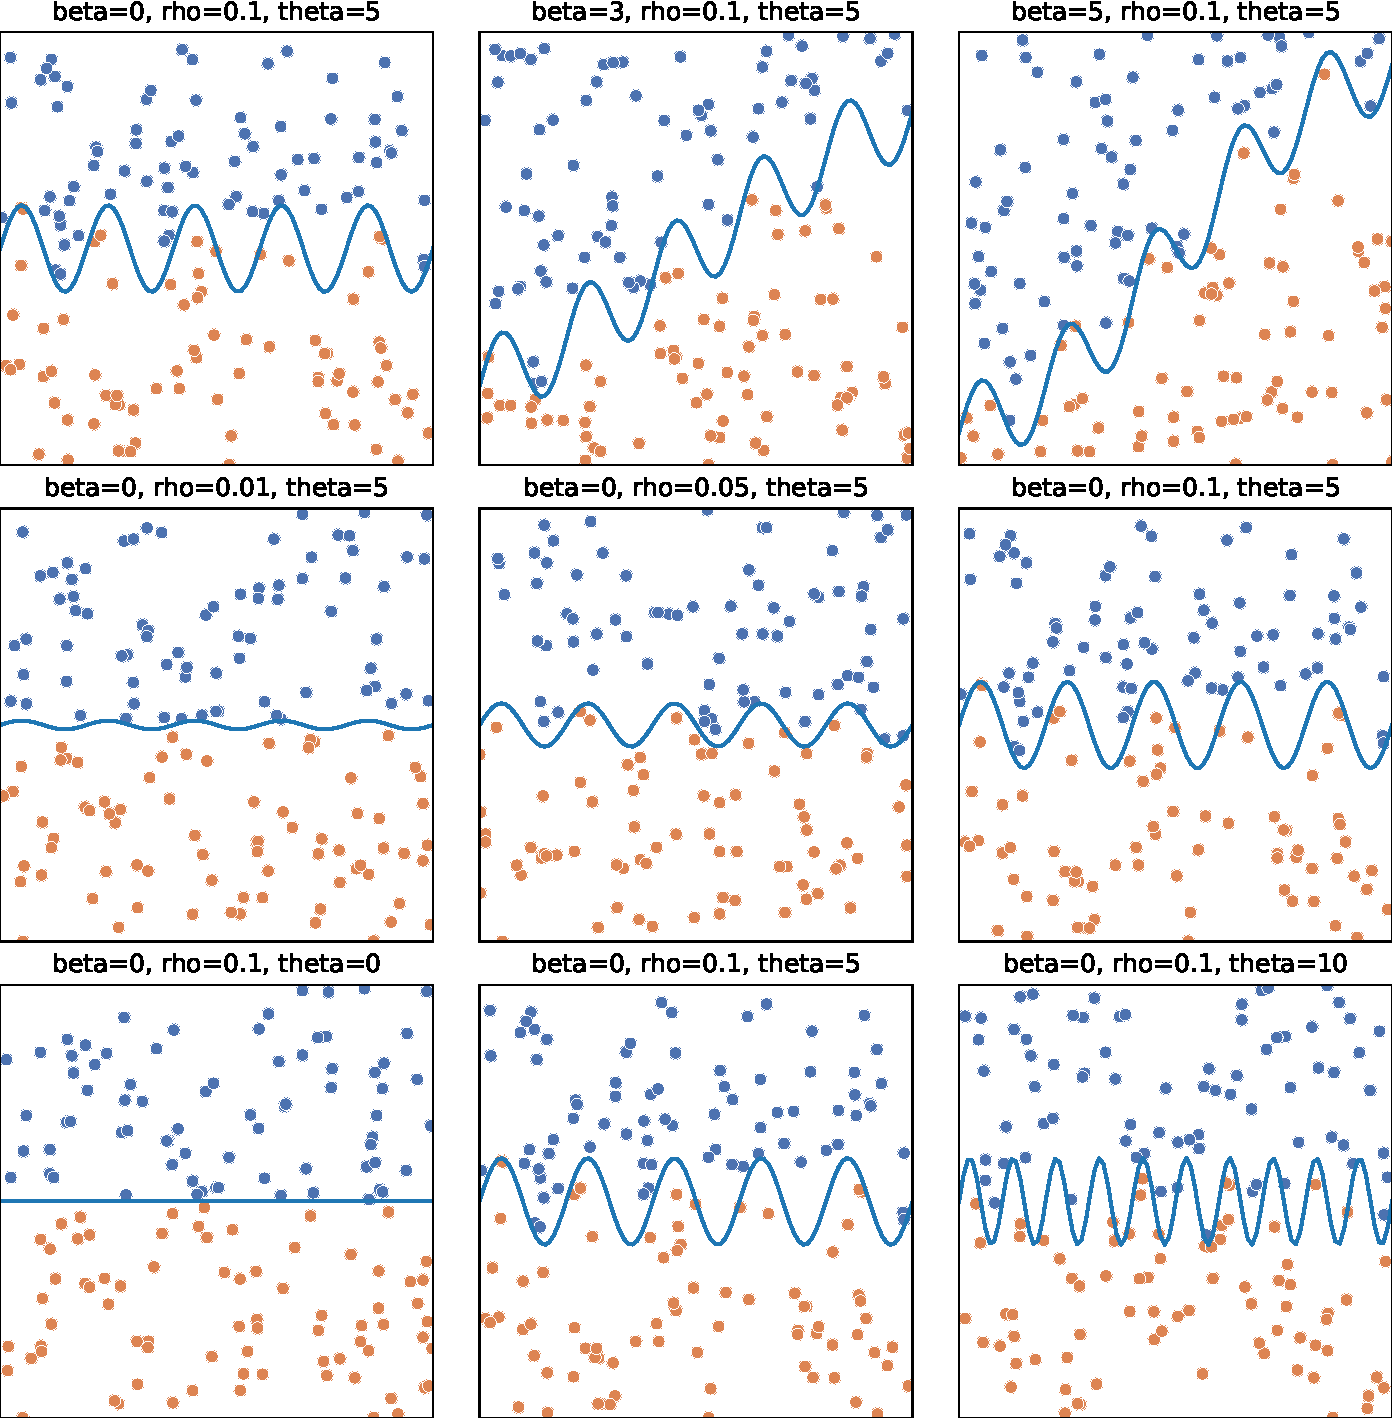
\includegraphics[width=1\linewidth]{img/sinusoid_dataset_param_influence.pdf}
    \caption{Esempio di dataset generati con funzione sinusoidale. 
    $\beta$ controlla ?, $\rho$ controlla l'ampiezza, $\theta$ la frequenza.}
    \label{fig:sinusoid_dataset}
\end{figure}

\subsubsection{Funzione paraboloide}
Fissati i parametri $\alpha, \text{x\_shift, y\_shift}$, per un vettore $\Vec{x}=\{x_1, \dots, x_n\} \in \mathrm{R}^n$, l'etichetta è calcolata con la funzione
$$
lf(\Vec{x})= x_n - \sum_{i=1}^{n-1}\alpha(x_i - \text{x\_shift})^2 - \text{y\_shift}.
$$
$\alpha$ controlla l'ampiezza del paraboloide, mentre x\_shift e y\_shift traslano il vertice del paraboloide.
La~\cref{fig:pacman_dataset} mostra alcuni esempi di dataset e funzioni di etichettatura al variare dei parametri.

\begin{figure}[ht]
    \centering
    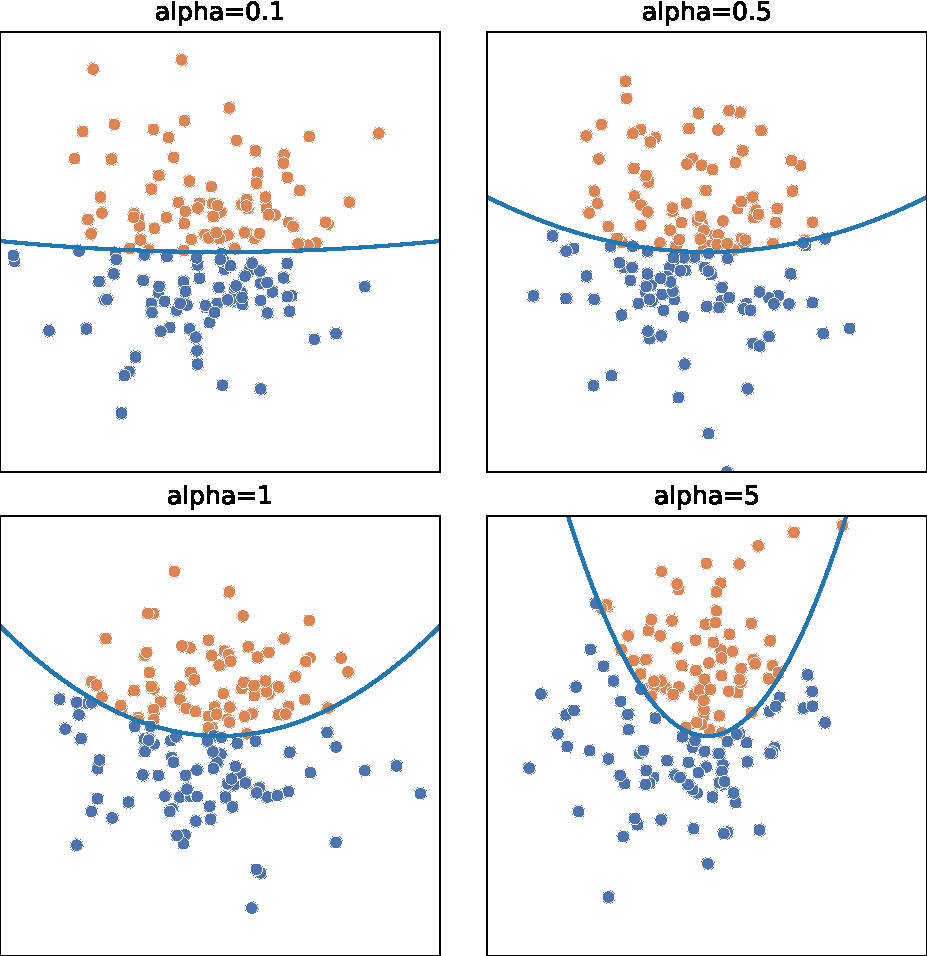
\includegraphics[width=1\linewidth]{img/pacman_dataset_param_influence.pdf}
    \caption{Esempio di dataset etichettati con paraboloide. $\alpha$ controlla l'ampiezza.}
    \label{fig:pacman_dataset}
\end{figure}

\subsection{Dataset reali}

\section{Esperiment su dataset sintetici 2D}

\subsection{Esperimenti su dataset con rumore}

\section{Esperiment su dataset sintetici 3D}

\section{Esperiment su dataset reali}

\section{Comparazione con altri metodi}









